\documentclass[a4paper]{article}
\usepackage[utf8]{inputenc}
\usepackage{fancyhdr}
\usepackage{amsmath}
\usepackage{tikz}
\pagestyle{fancy}

\usetikzlibrary{automata, positioning, arrows}

\setlength{\parindent}{0pt}
\setlength{\parskip}{1ex}

% Kopfzeile
\lhead{Optimierung B}
\chead{Übung 2}
\rhead{Niklas Fischer 298418 \\ Gereon Kremer 288911}

% Fußzeile
\lfoot{}
\cfoot{Seite \thepage{}}
\rfoot{}

\renewcommand{\thesection}{}
\renewcommand{\thesubsection}{(\alph{subsection})}

\begin{document}

\section{Aufgabe 1}
\subsection{}
Das ist im Allgemeinen falsch, wie das folgende Beispiel zeigt.

\[
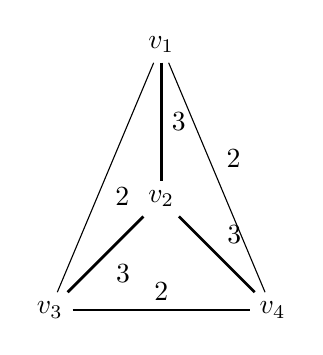
\begin{tikzpicture}[auto, node distance=2cm, baseline=-10ex]
	\node (v1) {$v_1$};
	\node (v2) [below=1.5cm of v1] {$v_2$};
	\node (v3) [below left of=v2] {$v_3$};
	\node (v4) [below right of=v2] {$v_4$};
	\path
		(v1) edge [line width=1pt] node {3} (v2)
		(v1) edge node {2} (v3)
		(v1) edge node {2} (v4)
		(v2) edge [line width=1pt] node {3} (v3)
		(v2) edge [line width=1pt] node {3} (v4)
		(v3) edge node {2} (v4)
	;
\end{tikzpicture}
\xrightarrow{c \rightarrow c^2}
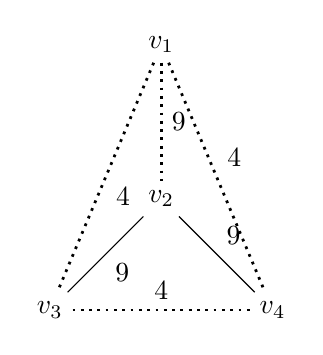
\begin{tikzpicture}[auto, node distance=2cm, baseline=-10ex]
	\node (v1) {$v_1$};
	\node (v2) [below=1.5cm of v1] {$v_2$};
	\node (v3) [below left of=v2] {$v_3$};
	\node (v4) [below right of=v2] {$v_4$};
	\path
		(v1) edge [line width=1pt, dotted] node {9} (v2)
		(v1) edge [line width=1pt, dotted] node {4} (v3)
		(v1) edge [line width=1pt, dotted] node {4} (v4)
		(v2) edge node {9} (v3)
		(v2) edge node {9} (v4)
		(v3) edge [line width=1pt, dotted] node {4} (v4)
	;
\end{tikzpicture}
\]

\subsection{}
Auch dies ist mit dem selben Beispiel falsch.

\[
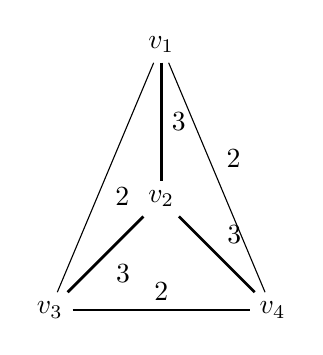
\begin{tikzpicture}[auto, node distance=2cm, baseline=-10ex]
	\node (v1) {$v_1$};
	\node (v2) [below=1.5cm of v1] {$v_2$};
	\node (v3) [below left of=v2] {$v_3$};
	\node (v4) [below right of=v2] {$v_4$};
	\path
		(v1) edge [line width=1pt] node {3} (v2)
		(v1) edge node {2} (v3)
		(v1) edge node {2} (v4)
		(v2) edge [line width=1pt] node {3} (v3)
		(v2) edge [line width=1pt] node {3} (v4)
		(v3) edge node {2} (v4)
	;
\end{tikzpicture}
\xrightarrow{X = \{v_2\}}
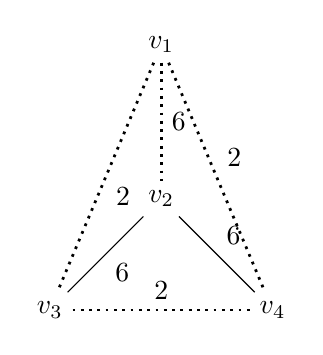
\begin{tikzpicture}[auto, node distance=2cm, baseline=-10ex]
	\node (v1) {$v_1$};
	\node (v2) [below=1.5cm of v1] {$v_2$};
	\node (v3) [below left of=v2] {$v_3$};
	\node (v4) [below right of=v2] {$v_4$};
	\path
		(v1) edge [line width=1pt, dotted] node {6} (v2)
		(v1) edge [line width=1pt, dotted] node {2} (v3)
		(v1) edge [line width=1pt, dotted] node {2} (v4)
		(v2) edge node {6} (v3)
		(v2) edge node {6} (v4)
		(v3) edge [line width=1pt, dotted] node {2} (v4)
	;
\end{tikzpicture}
\]

\subsection{}
Und auch diese Aussage ist falsch.

\[
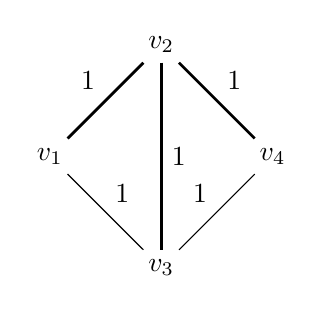
\begin{tikzpicture}[auto, node distance=2cm, baseline=0ex]
	\node (v1) {$v_1$};
	\node (v2) [above right of=v1] {$v_2$};
	\node (v3) [below right of=v1] {$v_3$};
	\node (v4) [below right of=v2] {$v_4$};
	\path
		(v1) edge [line width=1pt] node {1} (v2)
		(v1) edge node {1} (v3)
		(v2) edge [line width=1pt] node {1} (v3)
		(v2) edge [line width=1pt] node {1} (v4)
		(v3) edge node {1} (v4)
	;
\end{tikzpicture}
\xrightarrow{X = \{v_2, v_3\}}
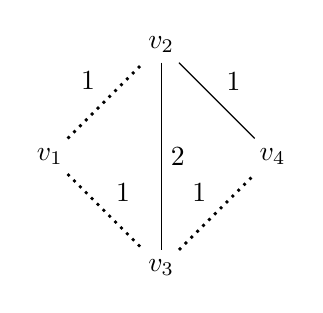
\begin{tikzpicture}[auto, node distance=2cm, baseline=0ex]
	\node (v1) {$v_1$};
	\node (v2) [above right of=v1] {$v_2$};
	\node (v3) [below right of=v1] {$v_3$};
	\node (v4) [below right of=v2] {$v_4$};
	\path
		(v1) edge [line width=1pt, dotted] node {1} (v2)
		(v1) edge [line width=1pt, dotted] node {1} (v3)
		(v2) edge node {2} (v3)
		(v2) edge node {1} (v4)
		(v3) edge [line width=1pt, dotted] node {1} (v4)
	;
\end{tikzpicture}
\]

\section{Aufgabe 2}

\begin{tabular}{l|l|l|l|l|l|l|l|l}
	& $x_1$ & $x_2$ & $x_3$ & $x_4$ & $x_5$ & $x_6$ & $x_7$ & $x_8$ \\
\hline
init	& $0$ & $\infty$ & $\infty$ & $\infty$ & $\infty$ & $\infty$ & $\infty$ & $\infty$ \\
\hline
$x_1 \xrightarrow{1} x_8$	& $0$ & $\infty$ & $\infty$ & $\infty$ & $\infty$ & $\infty$ & $\infty$ & $1$ \\
\hline
$x_1 \xrightarrow{2} x_2$	& $0$ & $2$ & $\infty$ & $\infty$ & $\infty$ & $\infty$ & $\infty$ & $1$ \\
\hline
$x_1 \xrightarrow{2} x_7$	& $0$ & $2$ & $\infty$ & $\infty$ & $\infty$ & $\infty$ & $2$ & $1$ \\
\hline
$x_1 \xrightarrow{3} x_5$	& $0$ & $2$ & $\infty$ & $\infty$ & $3$ & $\infty$ & $2$ & $1$ \\
\hline
$x_2 \xrightarrow{1} x_3$	& $0$ & $2$ & $3$ & $\infty$ & $3$ & $\infty$ & $2$ & $1$ \\
\hline
$x_8 \xrightarrow{2} x_6$	& $0$ & $2$ & $3$ & $\infty$ & $3$ & $3$ & $2$ & $1$ \\
\hline
$x_8 \xrightarrow{4} x_4$	& $0$ & $2$ & $3$ & $5$ & $3$ & $3$ & $2$ & $1$ \\
\hline
\end{tabular}

\section{Aufgabe 3}

\section{Aufgabe 4}

\end{document}
